\documentclass{beamer}

% \usepackage{beamerthemesplit} // Activate for custom appearance

\title{OTA Updates for an IOT Security Device}
\author{Aneesh Malhotra, Ryan Thomas, Sohail Iqbal, Gerson Dalton, Mohammad Nur}
\date{\today}

\usetheme{Singapore}
\usepackage{siunitx}
\begin{document}

\frame{\titlepage}

\section[Outline]{}
\frame{\tableofcontents}

\section{Introduction of Problem}
\subsection{}
\frame
{
  \frametitle{Introduction}
  
  \begin{itemize}
  \item FPGA's can be used to enhance security in wireless sensor networks by implementing a cryptographic exchange between wireless nodes in a network. 
  \item Advancements in network attacks, however, could potentially leave these systems vulnerable. 
  \item In the event the system is compromised it may be necessary to implement a firmware update. 
  \item Over-the-air updates are those that occur wirelessly, and allow the system to be updated easily without disassembly. 

  \end{itemize}
}

\frame{
\frametitle{Functionality}

\begin{itemize}
\item Our plan is to improve upon an FPGA enhanced sensor network, allowing for OTA -update capability.
\item Updates could be used to update security or provide additional functionality to the system. 
\item These firmware updates must include the microcontroller and FPGA in each sensor node. 
\item This additional functionality must be able to implemented securely without creating potential vulnerabilities.
\end{itemize}
}

\section{Top-Level Design}

\frame{
\frametitle{Top Level Design}
\begin{enumerate}
\item The update will be located in the cloud (Dropbox).
\item The app will include an update button that instructs the system to push the update. 
\item XBee will push the update the update to the MSP, which will calculate the size of the update and break it apart into components while pushing it to a memory pool.
\item The MSP then takes update data from memory and pushes it to the FPGA. 
\end{enumerate}
}

\section{Top-Level Design}

\frame{
\frametitle{Top Level Design}
\begin{figure}[!ht]
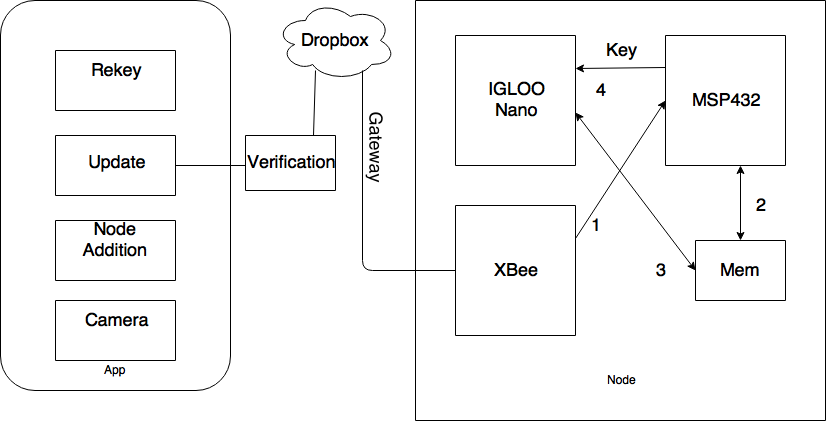
\includegraphics[scale = 0.35]{Diagram1.png}
\caption{Top Level Design of OTA Update system}
\end{figure}
}
\section{FPGA}
\frame{
\frametitle{FPGA}
\begin{figure}[!ht]
\centering
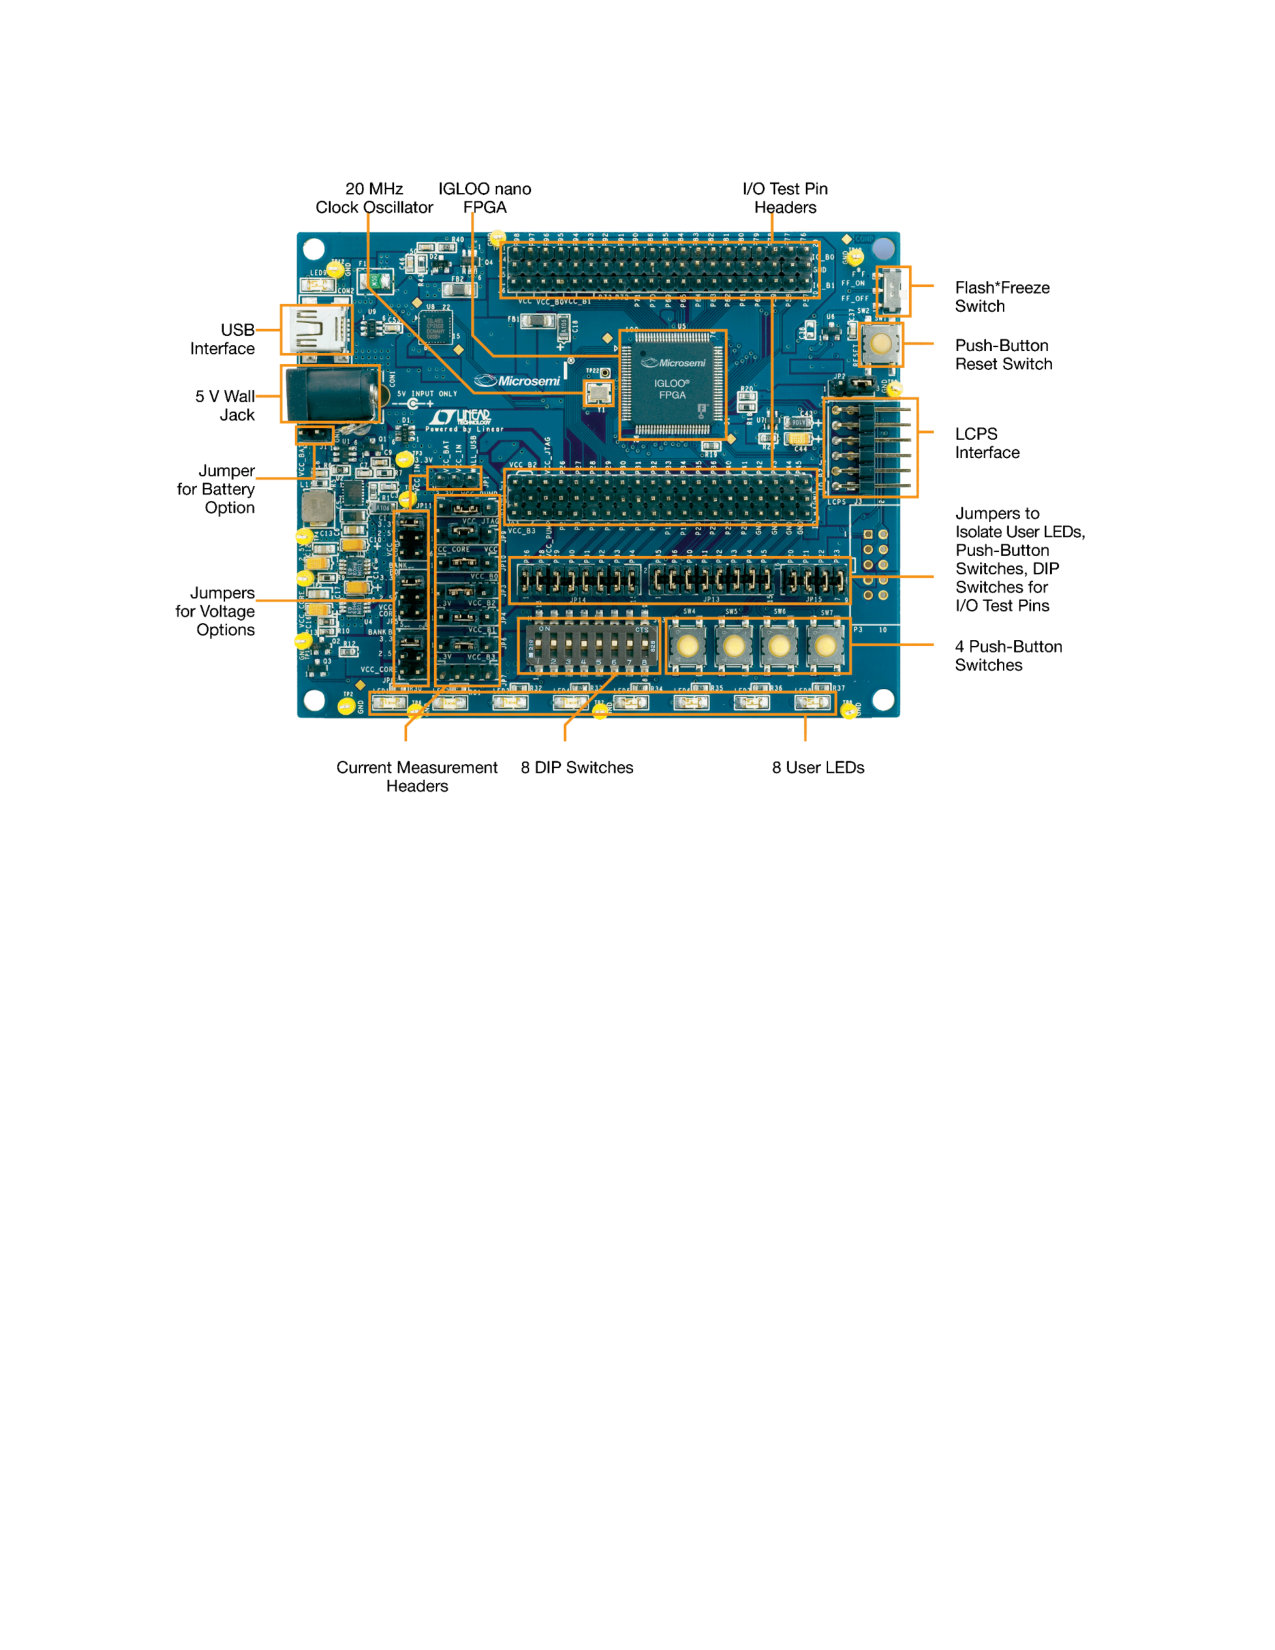
\includegraphics[scale=0.5]{igloo.pdf}
\caption{ACTEL Igloo Nano}
\end{figure}
}


\frame{
\frametitle{FPGA}
\begin{figure}[!ht]
\centering
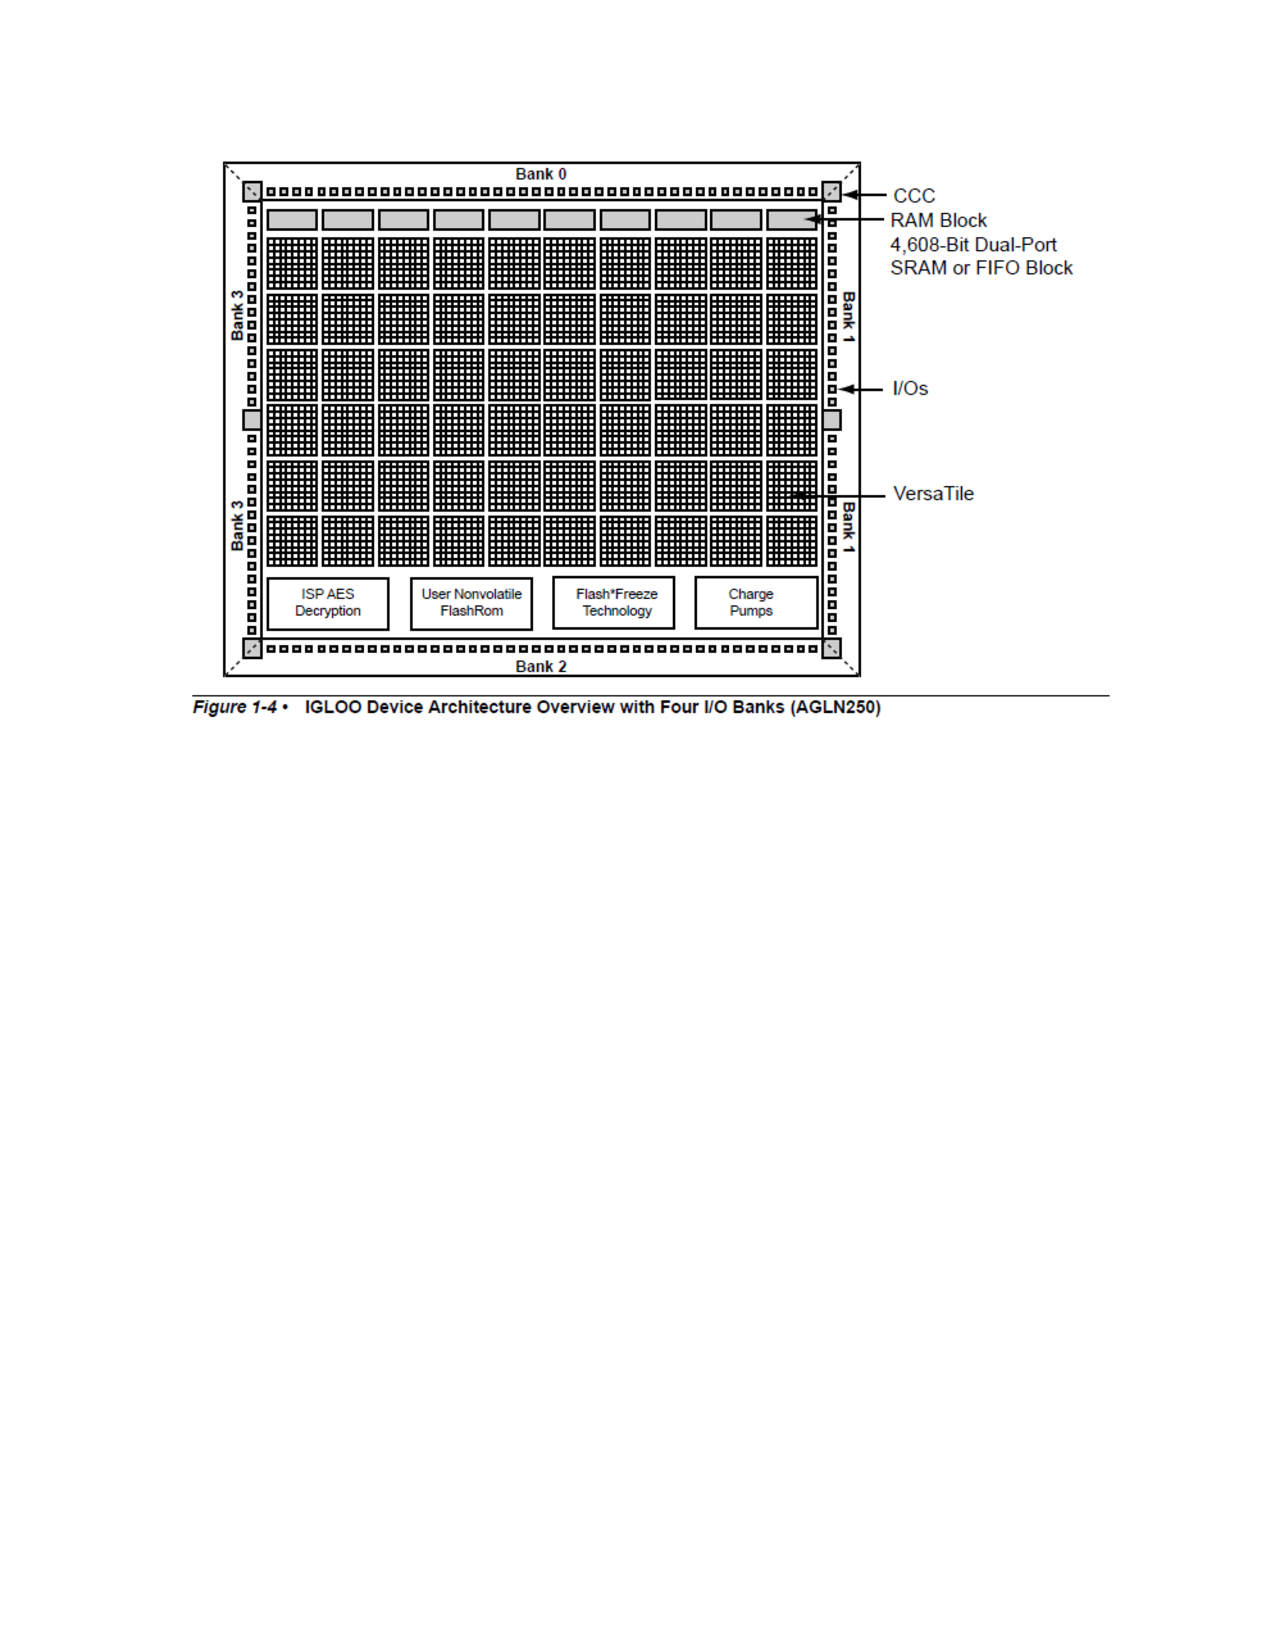
\includegraphics[scale=0.5]{igloo2.pdf}
\caption{ACTEL Igloo Nano}
\end{figure}
}
\frame{
\frametitle{FPGA}
\begin{itemize}
\item The IGLOO nano contains $1\si{kbit}$ of \textit{nonvolatile} Flash ROM memory. 
\item ROM is written using IGLOO nano IEEE 1532 JTAG programming interface. It's content can be read back using the JTAG programming interface or via direct FPGA core addressing.
\item The core can be individually programmed (erased and written), and on-chip AES decryption can be used selectively to securely load data over public networks with the security key stored in Flash ROM. 
\item IGLOO nano devices have embedded SRAM blocks which are $4608\si{bits}$ in size, and have independent read/write ports whose bit widths can be configured.
\end{itemize}
}

\frame{
\frametitle{FPGA Specifications}
\begin{itemize}
\item Clock Conditioning Circuit (CCC) and PLL
\begin{enumerate}
\item Up to six CCC blocks, one with an integrated PLL
\item Configureable Phase Shift, Multiply/Divide, Delay
\item Wide input frequency range ($1.5 \si{MHz} - 250 \si{MHz}$)
\end{enumerate}
\item Embedded Memory
\begin{enumerate}
\item 1kbit of Flash ROM non-volatile memory
\item SRAM's and FIFO's with Variable-Aspect-Ratio.
\item 4608 bit RAM
\item Blocks (x1,x2,x4,x9,x18) organizations
\item True Dual-Port SRAM (except x18 organization)
\end{enumerate}
\end{itemize}
}

\section{Data Protocols and Memory}
\frame{
\frametitle{Data Protocols}
\begin{itemize}
\item Our wireless sensor node will use the MSP432, which is a low power microcontroller for processing and redirecting sensor data.
\item The FPGA can be made handle the same data protocols as the MSP432 such as $\text{I}^2\text{C}$, SPI, and UART.
\item $\text{I}^2\text{C}$ and UART protocols require 2 pins, while SPI requires 4.
\item $\text{I}^2\text{C}$ and SPI are synchronous transfers, whereas UART is asynchronous and does not require a clock.
\item SPI can transfer at 16Mbps
\item UART can transfer at 960kBps
\end{itemize}

}

\frame{
\frametitle{Memory}
\begin{itemize}
\item The MSP432 has $64 \si{kB}$ RAM.
\item Both the MSP432 and FPGA have $256 \si{kB}$ of flash memory.
\item The size of the current system is $222 \si{kB}$, and the picture size is a maximum of $60 \si{kB}$
\item In order to be able able to support an update we need to have an external memory pool.
\end{itemize}

}



\section{Zigbee}
\frame{
\frametitle{Zigbee}
\begin{itemize}
\item A high level communication protocol based in IEEE 802.15.4, which is used in low rate wireless personal networks. 
\item Zigbee is common in IoT devices as an alternative to WiFi.
\end{itemize}
}
\frame{
\frametitle{Pros of Zigbee}
\begin{itemize}
\item It is designed for small devices for low power consumption.
\item It is a mesh network standard which can use other devices to pass signals over long distances.
\item The data rates vary from $20 \si{kbps} - 250 \si{kbps}$ in the $2.4 \si{GHz}$ band.
\item Has good performance in environments with low SNR. 
\item Secures data through 128-bit symmetric encryption keys. 
\item Needs less than $64 \si{kb}$ of ROM and $2-32 \si{kb}$ of RAM. 
\end{itemize}
}

\section{Security}

\frame{
\frametitle{Encryption/Security}
\begin{itemize}
\item OTA update capability can provide a potential vulnerability to the system.
\item We need a system of authenticating updates as to prevent the system using a false update. 
\item We can do this using a digital signature or cryptographic hash function.
\end{itemize} 
}






\end{document}
